\chapter{Understanding Auxiliary Tasks for Value Function Learning}
\label{chap:understanding}

\begin{quote}
    This chapter is based on \longfullcite{voelcker2024when}.
\end{quote}

\section{Introduction}

As the previous chapter shows, end-to-end critic training can cause problems with learning good intermediate neural network representations.
While regularization can alleviate some of the optimization failures, it only addresses issues of divergence, and does not ensure that relevant information is properly represented in a decision-aware fashion.
To achieve this, we now take a look at \emph{auxiliary tasks} which directly ensure that transition information is well represented in learned features.

Since the emergence of deep learning, techniques for deep supervised learning have been successfully incorporated into reinforcement learning (RL) agents \parencite{dqn,ddpg}.
However, as we have seen, the RL setting contains additional complications such as non-stationary optimization target and the reliance on bootstrapping.
These hurdles generally add instability to the RL training process, and as discussed, \emph{the failure to learn good features} is a central problem in deep RL \parencite{kumar2021implicit,lyle2022understanding,nikishin2022primacy,hussing2024dissecting}.

To mitigate this failure, one common approach is to add auxiliary tasks to the learning objective \parencite{jaderberg2017reinforcement}. 
Popular examples include predicting next state observations \parencite{jaderberg2016reinforcement} and predicting functions of the next state, or latent self-prediction, \parencite{schwarzer2021dataefficient,ni2024bridging}.
To understand the performance of these approaches, recent literature \parencite{tang2022understanding,lelan2023bootstrapped} considers the \emph{learning dynamics} of auxiliary task learning in simple linear surrogate models \parencite{saxe2014exact}.
Findings in the literature show that observation reconstruction should provide better features than latent self-prediction \parencite{behzadian2019fast,tang2022understanding}. 
However, this causes a theory-practice gap as empirical work has found that latent self-prediction outperforms observation reconstruction across many benchmarks \parencite{schwarzer2021dataefficient,ni2024bridging}.
This suggests that the assumptions made in \textcite{behzadian2019fast,tang2022understanding} might not match the setting that is commonly investigated in the empirical literature.

To address this gap, we pose two questions: \emph{(a) How do auxiliary losses behave when combined with a TD loss?} \textcite{tang2022understanding,lelan2022generalization,tang2023towards} have studied the learning dynamics of auxiliary tasks alone, evaluating their performance without addressing the interaction between the auxiliary task and the main goal, to learn a (correct) value function. \emph{(b) How can we describe the behavior of auxiliary losses in the presence of distractions (states and transition dynamics irrelevant for the reward) and observation functions (different ways to measure the underlying state)?} \ac{mdp}  structures like distractions have been hypothesized to lead to differing performance between different auxiliary tasks \parencite{ni2024bridging}, but to our knowledge no theoretical study has been established.


\autoref{sec:understanding:background} we briefly review notation and provide a formal model of the studied representation losses.
In \autoref{sec:understanding:formalism}, we present a formalization of distractions and observation functions. We use the framework of \emph{factored MDPs} \parencite{boutilier2000stochastic} with Kronecker products \parencite{mahadevan2009learning} to represent a common class of distractions. To model observation functions, we use \emph{linear reparametrization} as a tractable way to go beyond one-hot representations. 

In \autoref{sec:understanding:stand_alone_tasks} and \autoref{sec:understanding:auxilliary_tasks} we analyze the features learned with observation prediction and latent self-prediction alone and in combination with TD learning. 
We also show how these stationary features change with the introduction of distractions and observation functions.
From this analysis we find that latent self-prediction is a strong \emph{auxiliary task}, while observation prediction is a strong feature learning method when used \emph{alone}.
The differences are highlighted in \autoref{fig:understanding:losses}.
This bridges one of the biggest gaps between previous analysis of learning dynamics and empirical results.

In \autoref{sec:understanding:empirical} we test the predictions derived from our theoretical framework by evaluating feature learning losses in the MinAtar suite \parencite{young19minatar}\footnote{All code for our experiments is available at \url{https://github.com/adaptive-agents-lab/understanding_auxiliary_tasks}.}.
We design ablations that mirror both our formalization and previous approaches to test distraction robustness in empirical environments. 
The theory partially predicts the performance differences in the test suite, validating that the insights we obtain from the simple linear surrogate models used for analysis are useful for practitioners.
However, as we have an incomplete understanding of the underlying benchmark problems themselves \parencite{voelcker2024can}, more research is needed to fully characterize the interaction of the environment dynamics with the stabilizing auxiliary tasks.

\begin{figure}
    \centering
    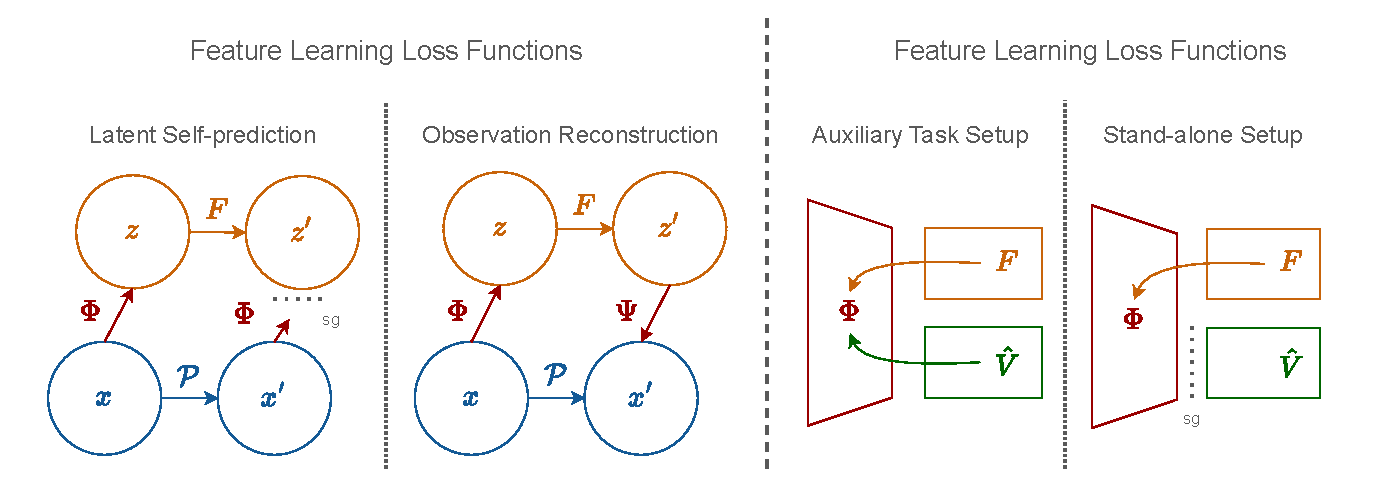
\includegraphics[width=\textwidth]{illustrations/thesis_understanding_overview.pdf}
    \caption{Diagram of the discussed loss functions and use cases. In latent self-prediction, we aim to predict the next state's \emph{features}, computed with an embedding function $\phi(x')$ using the state's features $\phi(x)$ and a latent prediction model $F$. In observation reconstruction, the next state's \emph{ground truth observations} $x'$ are matched via the use of a decoder function $\psi(F(\phi(x)))$. In the \emph{auxiliary task setup}, both the gradients from the feature learning loss and value function learning are propagated to the encoder, while in the \emph{stand-alone scenario}, only the gradients from the feature learning loss are used to update $\Phi$.}
    \label{fig:understanding:losses}
\end{figure}

\section{Mathematical formalism for analysis}
\label{sec:understanding:background}

In this chapter, we will focus on learning in finite state-action problems.
However, our approximations will not be tabular, as discussed in \autoref{chap:background}, but two layer linear networks.
This allows us to discuss the mechanisms underlying representation learning in a tractable setting.
We will generally assume that our states are represented by one-hot vectors.

\subsection{Linear networks as analytical models for training dynamics}

Rigorously analyzing the effect of different loss functions on neural networks is challenging due to non-linearities in the networks, shifting data distributions, and policy updates.
Therefore, we have to resort to studying simplified models to obtain quantitative and qualitative results, and only consider policy evaluation in our analysis.
Studying feature learning dynamics using linear networks was popularized by \textcite{saxe2014exact} and has proven to be a valuable tool to analyze diverse objectives such as TD learning \parencite{tang2023towards,lelan2023bootstrapped}, latent self-prediction \parencite{tian2021understanding,tang2022understanding}, and linear auto-encoders \parencite{pretorius2018learning,bao2020regularized}.

We rewrite the feature learning algorithms using two to three matrices in lieu of more complex functions. 
The embedding function or encoder $\Phi \in \mathbb{R}^{n \times k}$ projects the one-hot encoded state $x$ into a $k$ dimensional embedding space,
$F \in \mathbb{R}^{k\times k}$ is a \emph{latent model} or transition function mapping the embedded state to the next state's latent embedding.
$\hat{V} \in \mathbb{R}^{k}$ and $\hat{r} \in \mathbb{R}^{k}$ \emph{value and reward functions}, which operate in the latent space.
Finally, for the reconstruction loss, $\Psi \in \mathbb{R}^{k \times n}$ is a \emph{decoder} which maps from the latent space back to the ground truth observation space.

Furthermore, we use a simplifying assumption on the dataset and the embedding function throughout this chapter.
\begin{assumption}
\label{assumption:understanding:1}
Assume that $\Phi$ has maximal rank at initialization.
Assume that the dataset of states $\mathcal{D}$ is uniform i.i.d. over the state space and fixed throughout learning.
\end{assumption}
While uniform i.i.d. is a potentially optimistic assumption, we make it here to avoid dealing with questions of exploration and unvisited states.
Instead, we could have also assumed that the states are distributed according to the stationary distribution under the fixed policy.
However, as the results presented in \textcite{ghosh2020representations} (discussed in detail in \autoref{sec:understanding:auxilliary_tasks}) show, latent self-prediction based features guarantee stable convergence of the TD loss independent of the sampling distribution (as long as all states have non-zero probability in the dataset).

With these assumptions, and the fact that we represent state as one hot vector, we can use the fact that the covariance of the state features becomes $$\mathbb{E}_{x\sim \mathcal{D}}[xx^T] = I.$$
This simplifies notation throughout this chapter.

Using our set of assumptions, we study four important loss functions for RL: observation reconstruction, where the aim is to fit the next state observation $x^\top \Phi F \Psi \approx x'$, latent reconstruction $x^\top \Phi F \approx x' \Phi$, where the aim is to predict learned features of the next state, and TD learning $x^\top \Phi \hat{V} \approx x^\top(r^\pi + \gamma x'^\top\phi \hat{V})$. To clarify the differences, we show a diagram explaining the losses and training setups in \autoref{fig:understanding:losses}.
Following common notation, $[\cdot]_\mathrm{sg}$ signifies a \emph{stop-gradient} operation; no gradient is taken with regard to terms in the parenthesis.

Formally, these are written as
\begin{align}
    \text{Reconstruction: }&& L_{\text{rec}}(\Phi,F,\Psi) =& \,\EEX{x \sim \mathcal{D}}{\ltwonorm{x^\top \Phi F \Psi - x^\top {P^\pi}}^2},\\
    \text{Latent self-prediction: }&& L_{\text{lat}}(\Phi,F) =& \,\EEX{x \sim \mathcal{D}}{\ltwonorm{x^\top \Phi F - \left[x^\top {P^\pi} \Phi\right]_{\mathrm{sg}}}^2}, \\
    \text{TD Learning: }&& L_{\text{td}}(\Phi,\hat{V}) =& \,\EEX{x \sim \mathcal{D}}{\ltwonorm{x^\top \Phi \hat{V} - \left[x^\top  \left(r^\pi + \gamma P^\pi \Phi \hat{V}\right)\right]_{\mathrm{sg}}}^2}.
\end{align}

Following the nomenclature of this thesis, we refer the first two losses as \emph{general-purpose}, and TD-learning as \emph{decision-aware} as it depends on information specific to the decision problem.
To analyze the discrete-time learning dynamics, we study the analogous continuous-time gradient flow, which allows us to use the toolkit of dynamical systems theory.
Writing $\alpha_\Phi$ and $\alpha_F$ for the representation and model learning rates, i.e., the latent self-prediction dynamics are
\begin{align}
    \ddt{t} \Phi_t &= -\alpha_\Phi\nabla_{\Phi_t} {L}_{\text{lat}}(\Phi_t, F_t) = -2 \alpha_\Phi (\Phi_t F_t - P^\pi \Phi_t)  F_t^\top,\\
    \ddt{t} F_t  &= -\alpha_F\nabla_{F_t} {L}_{\text{lat}}(\Phi_t, F_t) = -2 \alpha_F \Phi_t^\top(\Phi_t F_t - P^\pi \Phi_t).
\end{align}

We primarily consider the \emph{two-timescale} regime, i.e. the assumption that $\alpha_F\to \infty$ \parencite{tang2022understanding}. 
Intuitively, this describes a learning setup in which the latent model is learned ``much faster'' than the latent mapping. 
This guarantees the non-collapse property for $\Phi$, which means that the inner product $\Phi^\top\Phi = C$ is constant throughout training \parencite{tang2022understanding}.
In addition, as we are operating in the gradient flow limit, we will set $2\alpha_\Phi = 1$ throughout this chapter.
This results in the following dynamics for self-predictive learning:
\begin{equation}
    \label{eq:understanding:BYOLTwoTimescale}
    F_t^* = \left(\Phi_t^\top\Phi_t\right)^{-1} \Phi_t^\top P^\pi \Phi_t, \quad \frac{d}{dt}\Phi_t = \left(I-\Phi_t\left(\Phi_t^\top \Phi_t\right)^{-1}\Phi_t^\top\right)P^\pi \Phi_t {F_t^*}^\top,
\end{equation}
where our assumption on the initialization of $\Phi$ and the non-collapse property guarantee that the inverse exists $\left(\Phi_t^\top\Phi_t\right)^{-1}$.

\section{Formalizing distractions and observation functions}
\label{sec:understanding:formalism}
To bridge the theory-practice gap in feature learning, we formalize two structures of MDPs commonly found in Deep RL benchmarks that have, to the best of our knowledge, not appeared in work analyzing feature learning: observation functions and distractions.
To allow a close comparison with previous work, our changes to the formalism are minimal on purpose, while still highlighting the important role these changes play in different loss functions.

\subsection{Observation functions}
Previous literature \parencite{tang2022understanding,tang2023towards,lelan2022generalization} has eschewed the underlying observation of states in their analysis of representation dynamics. 
The assumption that $x$ is represented by a one-hot vector, which we have made explicit above, implies that the features for the underlying states can be learnt independently.
With a one-hot representations, the features of $x$ are simply $x^\top \Phi = \Phi[i]$, the $i$-th row of $\Phi$.
A more realistic setting, which we focus on in \autoref{sec:understanding:observation}, is considering observation functions acting on the underlying states. 
This allows for representing systems where some states have correlated observations, which may be helpful \emph{or} harmful for the RL problem. 

We briefly state this for reference later.
\begin{assumption}
    \label{assumption:understanding:2}
    Let an \emph{observation function} for a finite state space \ac{mdp} be an invertible matrix $\mathcal{O} \in \mathbb{R}^{n \times n}$.
    Assume that the reward is not affected by this introduction.
\end{assumption}

\textbf{Formalization:} To introduce an observation function while remaining in the regime of analyzing linear networks and finite state problems, each one of $n$ states is mapped to a unique $n-$dimensional observation vector by an invertible \emph{observation matrix} $\gO \in \vecR{n}{n}$.\footnote{We could also consider projection into higher dimensional spaces $\gO \in \vecR{n}{d}$ with $d > n$, without violating the Markov assumption, but this leads to additional complications (working with pseudo-inverses instead of inverses) which do not contribute meaningfully to the insights in this work.}

This change from one-hot vectors to arbitrary vectors allows us to account for similarities between different state observations.
For example, if two states have almost identical observation vectors, they will be mapped to similar points in the latent representation space unless the features directly counteract this.
We study the impact of changing the observations with a linear reparameterization in \autoref{sec:understanding:observation} by replacing $x$ with $\bar{x} = \mathcal{O}^\top x$.


\subsection{Distracting state dynamics}
In addition to observation functions, another common problem that many reinforcement learning algorithms face are distractions.
While distractions have been a focus of empirical work studying the relative efficacy of different auxiliary tasks \parencite{ni2024bridging}, a simple formalism whose effect on learning dynamics can be analyzed has not been presented. 
We propose to model an \ac{mdp}  with distractions using factored MDPs \parencite{boutilier2000stochastic}.

\begin{definition}[A factored \ac{mdp}  model of a distraction]\label{def:distracting}
Let $M=(\mathcal{M}, P_{M},R_M)$,  $N=(\mathcal{N},P_N,R_N)$ be a pair of Markov decision processes.
The product process $M \otimes N$ is a \ac{mdp}  with state space $\mathcal{M}\times \mathcal{N}$, transition kernel $P_M\otimes P_N$ (where $\otimes$ signifies the Kronecker product), and reward function $R_M\otimes \vone +\vone \otimes R_N^\top$.

If $R_N = 0$, we refer to $N$ as a distracting process, as it does not contribute to the reward.
\end{definition}

This process models a common occurrence: two non-interacting processes unfold simultaneously, with the states being a combination of the two.
Such a process can model some well-studied forms of distraction, such as the background distractions used in \textcite{stone2021thedc} or the random observation dimension used in \textcite{nikishin2021control} and the next chapter.
In this case, the foreground process $M$ is assumed to carry the reward information, while the reward vector of the background process $N$ is 0.
We review important properties of the Kronecker product in \autoref{app:formal:understanding:linalg}.


Note that our formalizations of observation functions and distracting processes is distinct from the assumptions in \emph{linear MDPs} \parencite{jin2020provably}. Concretely we do not assume that the processes are low-rank compressible, just that they are factorizable.

\section{Reconstruction and self-prediction losses}
\label{sec:understanding:stand_alone_tasks}

In this section and the next, we present an analysis of the stability conditions of reconstruction and self-prediction losses with linear networks.
Using this analysis, we obtain several \emph{insights}, qualitative predictions about how we expect the studied losses to behave in more complicated scenarios.
These \emph{insights} present the basis for our empirical comparison in \autoref{sec:understanding:empirical}.

\subsection{Case 1: Orthogonal state representations}


\textcite{tang2022understanding} show that for MDPs with symmetric transition kernels ($\mathcal{P}^\top = \mathcal{P}$), latent self-prediction converges to subspaces spanned by eigenvectors of $P^\pi$. 
We extend this result in the following sense: if $P^\pi$ has positive real eigenvalues, invariant sub-spaces which are not spanned by the top-k eigenvectors are unstable for gradient descent.\footnote{The assumption of real \emph{positive} eigenvalues is both more and less restrictive than the symmetry assumption made by \textcite{tang2022understanding}. An extension of our result to negative eigenvalues is presented below, together with an extended comparison to the results in \textcite{tang2022understanding} and \textcite{lelan2023bootstrapped}.}
Note that the resulting features are identical to those obtained from the random reward assumption described in \textcite{lelan2023bootstrapped} (albeit under slightly different technical conditions), which highlights the close connection between the self-predictive approach and bootstrapped generalized value function learning.
This furthermore suggests that using random rewards as auxiliary objectives \parencite{farebrother2023protovalue} should result in similar features to those obtained with self-prediction.

\begin{assumption}
\label{assumption:understanding:3}
    Assume a two-timescale scenario and that $F$ is initialized with full rank. 
    Hence the non-collapse property ($\Phi_t^\top\Phi_t = \Phi_0^\top\Phi_0$) \parencite{tang2022understanding} holds.
\end{assumption}
When referring to eigenvectors and singular vectors, we mean the \emph{right} vectors of the corresponding matrices unless stated otherwise.
We now present our first theoretical result.

\begin{restatable}[Stationary points of latent self-prediction]{proposition}{BYOLGradientFlow}\label{prop:understanding:1}
Assume \autoref{assumption:understanding:1} and \autoref{assumption:understanding:2} hold.
Furthermore, suppose $P^\pi$ is real-diagonalizable. 
If the columns of $\Phi_t$ span an invariant subspace of $P^\pi$, $\Phi_t$ is a stationary point of the dynamical system.
Furthermore, if $P^\pi$ is real-diagonalizable with positive eigenvalues, all invariant subspaces not spanned by the top-k eigenvectors sorted by eigenvalue are asymptotically unstable for gradient descent.
\end{restatable}

\begin{proof}
    At any stationary point the gradient $\frac{d}{dt}\Phi_t$ must be equal to $0$, which from \cref{eq:understanding:BYOLTwoTimescale} means that we must have $\left(\Phi_t\left(\Phi^\top_t \Phi\right)^{-1}\Phi_t^\top - I\right)P^\pi\Phi_t \Phi_t^\top {P^\pi}^\top \Phi_t\left(\Phi^\top_t \Phi\right)^{-\top}=0$.
    We will denote stationary points with $\Phi^*$.

    Assume that the column vectors of $\Phi^*$ spans an invariant subspace of $P^\pi$. This implies that there exists a full rank matrix $A$ so that $P^\pi \Phi^* = \Phi^*A$.
    Then 
    \begin{align}
    \left(\Phi^*\left({\Phi^*}^\top \Phi^*\right)^{-1}{\Phi^*}^\top - I\right)P^\pi\Phi^* F^*=\Big(\Phi^*\underbrace{\left({\Phi^*}^\top \Phi^*\right)^{-1}{\Phi^*}^\top\Phi^*}_{=I} - \Phi^*\Big)A F^*=0. \label{eq:understanding:stationary}
    \end{align}

This shows that $\frac{\mathrm{d}\Phi}{\mathrm{d}t} = 0$, which means that $\Phi^*$ is indeed a stationary point, which proves the first part of the proposition.

There are additional critical points of the differential equation, as discussed by \textcite{tang2022understanding}.
In the analysis of stability, we first show the case of critical points corresponding to the claim in the proposition.
We then briefly discuss other cases after the proof.

\textbf{Case 1: $\Phi_t$ spans an invariant subspace of $P^\pi$}
Invariant subspaces correspond to subspaces spanned by right eigenvectors of $P^\pi$.

We write $P$ for $P^\pi$ to reduce notational clutter.
Let $e_1,\dots,e_k$ be the eigenvectors corresponding to the $k$ largest eigenvalues of $P$.
Let $\Phi^*$ correspond to any set of $k$ eigenvectors of $P$. 

To show that all non top-$k$ eigenspaces are asymptotically unstable critical points of the differential equation defined by the gradient flow of $\Phi$.
To show this, we aim to show that there exists an eigenvector of the Jacobian with an eigenvalue larger than $0$.
For this, we construct the directional derivative at the critical point.
The directional derivative is the Jacobian vector product, which allows us to circumvent the need to work with higher order tensor derivatives.
We then proceed to show that there exists a direction which corresponds to the eigenvector of the Jacobian with positive eigenvalue.
This concludes the proof.
This technique closely follows the one used by \textcite{lelan2023bootstrapped}.

Assume $\mathrm{span}\{\Phi^*\} \neq \mathrm{span}\{e_1,\dots,e_k\}$. This implies that there exists at least one eigenvector $e_j \in \{e_1,\dots,e_k\}$ and $e_j \notin \mathrm{span}\{\Phi^*\}$, with corresponding eigenvalues $\lambda_j$.

Let $D_\Delta$ be the directional derivative of $\ddt{t} \Phi |_{\Phi=\Phi^*}$ in the direction $\Delta$.
We construct the directional derivative using the product rule (terms colored for ease of reading),
\begin{align}
D_\Delta \ddt{t} \Phi |_{\Phi=\Phi^*} = & -D_\Delta \left(\left(\Phi F^* - P \Phi\right) {F^*}^\top\right)|_{\Phi=\Phi^*}\\
     = & -{\color{uoftred}D_\Delta \left(\Phi F^* - P \Phi\right)|_{\Phi=\Phi^*}} {F^*}^\top - \left(\Phi^* F^* - P \Phi^*\right) {\color{uoftmagenta}D_\Delta {F^*}|_{\Phi=\Phi^*}}^\top.
\end{align}

For the directional derivative, we only consider directions that are orthogonal to $\Phi^*$, so ${\Phi^*}^\top\Delta = 0$. Then $\underbrace{P{\Phi^*} = {\Phi^*} A}_{\text{subspace condition}} \implies \Delta^\top P \Phi^* = 0.$
For the derivative with regard to $F^*$, we have
\begin{align}
    {\color{uoftmagenta}D_\Delta F^*|_{\Phi = \Phi^*}} =& D_\Delta \left(\Phi^\top \Phi\right)^{-1}\Phi^\top P \Phi\nonumber\\
    =& \left(D_\Delta \left(\Phi^\top \Phi\right)^{-1} \right) {\Phi^*}^\top P {\Phi^*} + \left({\Phi^*}^\top {\Phi^*}\right)^{-1} \left(D_\Delta \Phi^\top P \Phi  \right)\nonumber\\
    =& -\underbrace{(\Delta^\top \Phi^* + {\Phi^*}^\top \Delta)}_{=0}\left({\Phi^*}^\top {\Phi^*}\right)^{-2}{\Phi^*}^\top P {\Phi^*} + \left({\Phi^*}^\top {\Phi^*}\right)^{-1}\big(\underbrace{\Delta^\top P {\Phi^*}}_{=0} + {\Phi^*}^\top P \Delta\big)\nonumber\\
    =& \left({\Phi^*}^\top {\Phi^*}\right)^{-1}\left({\Phi^*}^\top P \Delta\right). \label{eq2}
\end{align}
Therefore, the first term in the second line is dropped, as well as the first term of the final summand.

Note that $F^* = \left({\Phi^*}^\top{\Phi^*}\right)^{-1} {\Phi^*}^\top P^\pi {\Phi^*} = \underbrace{\left({\Phi^*}^\top{\Phi^*}\right)^{-1} {\Phi^*}^\top {\Phi^*}}_{=I}\, \mathrm{diag}(\Lambda_i) = \mathrm{diag}(\Lambda_i)$, where $\Lambda_i$ is the set of eigenvalues corresponding to the eigenvectors in $\Phi^*$ and $\mathrm{diag}(\Lambda_i)$ is the diagonal matrix of eigenvalues corresponding to those eigenvectors spanned by $\Phi^*$.

This allows us to compute the remaining derivative,
\begin{align}
    &{\color{uoftred}D_\Delta \left(\Phi F^* - P \Phi\right)|_{\Phi=\Phi^*}}\, \mathrm{diag}(\Lambda_i)\\
    = & \left(\Delta\, \mathrm{diag}(\Lambda_i) + \Phi^*{\color{uoftmagenta} D_\Delta F^*}  - P\Delta \right)\,\mathrm{diag}(\Lambda_i)\\
    = & \left(\Delta\, \mathrm{diag}(\Lambda_i) + \Phi^*\left({\Phi^*}^\top {\Phi^*}\right)^{-1}{\Phi^*}^\top P \Delta  - P\Delta \right)\,\mathrm{diag}(\Lambda_i),
\end{align}
where we use the fact that $D_\Delta P\Phi^* = P D_\Delta \Phi^* = P \Delta$.

Finally, as $\Phi^*F^* = \Phi^* \mathrm{diag}(\Lambda_i) = P^\pi \Phi^*$, we obtain
\begin{align}
 D_\Delta \ddt{t} \Phi |_{\Phi=\Phi^*} =   -\left(\Delta\, \mathrm{diag}(\Lambda_i) + {\Phi^*}\left({\Phi^*}^\top \Phi^*\right)^{-1}{\Phi^*}^\top P \Delta  - P\Delta \right)\mathrm{diag}(\Lambda_i) \\- \underbrace{\left(\Phi^* F^* - P \Phi^*\right)}_{=0\,\text{see \autoref{eq:understanding:stationary}}}\left({\Phi^*}^\top P \Delta\right)^\top.
\end{align}


By the definition of the directional derivative as the Jacobian-vector product, we can now assert
\begin{align}
    \left(\ddt{\Phi} \ddt{t}\Phi |_{\Phi=\Phi^*}\right) \Delta = - \left(\Delta \mathrm{diag}(\Lambda_i) + \left(\Phi^*\left({\Phi^*}^\top {\Phi^*}\right)^{-1}{\Phi^*}^\top - I\right) P \Delta\right)\mathrm{diag}(\Lambda_i).
\end{align}

What remains to be shown is that there exist a direction which corresponds to a positive eigenvalue of the Jacobian of the dynamics.

Choose $\Delta = v_j u^\top$. Let $v_j$ be an eigenvector not in the span of $\Phi^*$ but in the top-k eigenvectors. Let  $\lambda_j$ be the corresponding eigenvalue. By our assumption before, there exist at least one eigenvalue $\lambda_i \in \Lambda_i$ so that $\lambda_j > \lambda_i$.

Note that $\left(\Phi^*\left({\Phi^*}^\top {\Phi^*}\right)^{-1}{\Phi^*}^\top - I\right) P v_j = \Big(\Phi\left({\Phi^*}^\top {\Phi^*}\right)^{-1}\underbrace{{\Phi^*}^\top v_j}_{0\, \text{by construction}} - I v_j\Big) \lambda_j = -\lambda_j v_j$ and therefore $\left(\Phi^*\left({\Phi^*}^\top \Phi^*\right)^{-1}{\Phi^*}^\top - I\right) P \Delta = -\Delta \lambda_j I.$

To simplify notation, we will write $\Lambda_i$ for $\mathrm{diag}(\Lambda_i)$ from now on as there is no risk of confusion.

\begin{align}
    -\left(\Delta \Lambda_i + \left(\Phi^*\left({\Phi^*}^\top \Phi^*\right)^{-1}{\Phi^*}^\top - I\right) P \Delta\right)\Lambda_i = &- \Delta \left(\Lambda_i - \lambda_j I\right) \Lambda_i\\
    = &-\Delta \left(\Lambda_i^2 - \lambda_j \Lambda_i\right) \\
    = &\Delta \left(\lambda_j \Lambda_i - \Lambda_i^2\right).
\end{align}

We can now choose $u$ so that it is any eigenvector of $\left(\lambda_j \Lambda_i - \Lambda_i^2\right)$. As this is a diagonal matrix, it is easy to see that if $\lambda_j > \lambda_i$ for any $\lambda_i$, the matrix will have a positive eigenvalue, meaning there exists a direction in which the critical point is unstable.
\end{proof}

\textbf{Case 2: Non-invariant subspace cases:} Not all critical points lie in invariant subspaces.
One such an alternative critical point is the case of $\Phi^\top P \Phi = 0$, and more generally, for each set of column vectors $\phi_i$ in $\Phi$, they needs to either be mapped to an invariant or an orthogonal subspace by $P^\pi$ to be stable.
In the orthogonal case, the Jacobian at the critical point becomes 0, meaning no conclusion about stability can be drawn from this analysis.
We do however conjecture that the non-invariant subspace critical points are also saddle-points or unstable solutions of the ODE, following the experimental evidence presented in \textcite{tang2022understanding}.

\textbf{Negative eigenvalues:} In case the matrix has negative eigenvalues, the stability conditions in the final step of the proof change. The matrix $\lambda_j\Lambda_i - \Lambda_i^2$ will not have negative eigenvalues if $\lambda_i$ is negative but $\lambda_j$ is positive. The ranking of stable points follows this slightly un-intuitive ordering: all negative eigenvalues sorted by absolute value followed by all positive eigenvalues sorted by absolute value.



Our proof implies that even without the assumptions of symmetry of $P^\pi$ required in \textcite{tang2022understanding}, the dynamics of latent self-prediction will tend to converge to invariant subspaces spanned by eigenvectors with large eigenvalues as other invariant subspaces are unstable.
This is important as these are most important for representing potential reward functions in the environment, at least without additional assumptions on reward structure, then smaller eigenvectors \parencite{lelan2023bootstrapped}. 

We can contrast this with the features learned by a reconstruction loss.
We write $\mathrm{span}(A)$ for both the span of the column vectors of $A$ or for the span of a set of vectors $A$, depending on context.
\begin{restatable}[Stationary points of reconstruction]{proposition}{ReconstructionStationaryPoints}\label{prop:understanding:2}
Assume \autoref{assumption:understanding:1} and \autoref{assumption:understanding:2} hold. Write $(u_1,\dots,u_n)$, $(v_1,\dots,v_n)$ for the left and right singular vectors of $P^\pi$ sorted in descending order by singular value. Any stationary point $(\Phi^*, F^*, \Psi^*)$ of $L_\text{rec}$ under the two timescale scenario satisfies $\mathrm{span}\,(\Phi^*)=\mathrm{span}\left(\{u_1,\dots,u_k\}\right)$, $\mathrm{span}\,({\Psi^*}^\top)=\mathrm{span}\left(\{v_1,\dots,v_k\}\right)$.
\end{restatable}
\begin{proof}
We first show that under the two timescale scenario, $F$ is stationary and therefore does not change the span of the critical points.

Due to the assumption of the two-timescale scenario, we compute $\Psi^*$ by solving the linear regression problem,
\begin{align}
    &&\ddt{\Psi^*} \lVert \Phi F\Psi^* - P \rVert_F^2 &= F^\top {\Phi}^\top ({\Phi}F\Psi^* - P)\\
    &&0 &=  F^\top {\Phi}^\top ({\Phi}F\Psi^* - P)\\
    \Leftrightarrow && B^* &= \left(F^\top {\Phi}^\top {\Phi}F\right)^{-1} F^\top \Phi^\top P = F^{-1}\left(\Phi^\top \Phi\right)^{-1} \Phi^\top P.
\end{align}

Plugging this solution back into the original equation, 
\begin{align}
    \lVert \Phi F\Psi^* - P \rVert_F^2 &= \lVert \Phi FF^{-1}\left(\Phi^\top \Phi\right)^{-1} \Phi^\top P - P \rVert_F^2\\
    &= \lVert \Phi \left(\Phi^\top \Phi\right)^{-1} \Phi^\top P - P \rVert_F^2,
\end{align}
we notice that $F$ cancels.
Therefore, the optimality conditions for $A$ follow from the Eckart-Young theorem, as presented in \autoref{lem:understanding:rrr}.
\end{proof}


Features of this form have been studied extensively and the convergence properties of linear auto-encoders are well understood \parencite{baldi1989neural,pretorius2018learning,bao2020regularized}.

\autoref{prop:understanding:1} and \autoref{prop:understanding:2} together show that there is a subtle but important difference between latent self-prediction and observation reconstruction: the features will converge to invariant subspaces in the former case, and to singular space in the latter case.
Note that if $P^\pi$ is a symmetric matrix, then the singular spaces and the invariant subspace spanned by top-k eigenvectors coincide and latent self-prediction and reconstruction converge to the same features \parencite{tang2022understanding}.

\textcite{behzadian2019fast} show that top $k$ singular vectors are optimal low-rank linear features when making no assumptions on the reward, meaning observation reconstruction should lead to the best features when considering the supremum over any bounded reward.
If eigenvectors and singular vectors differ, \textcite{behzadian2019fast} and \textcite{lelan2023bootstrapped} both highlight that singular vectors often lead to better performing features.

So far our results line up with previously presented theoretical works and do not shed additional light on the observed theory-practice gap.
However, the assumption (or rather lack of assumptions) on the MDP, the reward, and the observation structure will be crucial to understanding these results more deeply in the next sections.

\begin{tcolorbox}[boxrule=0.2mm,colback=white,colframe=uoftblue,boxsep=0pt,top=3pt,bottom=5pt]
\begin{insight}[Optimality of observation prediction] The features learned by observation prediction are in general superior to those of latent self-prediction, when using solely one of these as the loss function, and if no additional assumptions on the structure of the reward are made.
\label{insight:understanding:1}
\end{insight}
\end{tcolorbox}

\subsection{Case 2: Observation function dependence}
\label{sec:understanding:observation}

Recall that the gradient dynamics presented in \autoref{eq:understanding:BYOLTwoTimescale} and analyzed in \autoref{prop:understanding:1} and \autoref{prop:understanding:2} rely on the assumption that $\mathbb{E}[xx^\top] = I$.
We now use the idea of an observation matrix $\gO$ to account for problems in which the observation space creates similarities between features.
To do this, we simply replace every occurrence of $x^\top$ in the losses presented in \autoref{sec:understanding:background} with $x^\top \gO$.
We assume that $x$ is a one-hot vector as discussed before and the coverage is still uniform (\autoref{assumption:understanding:1} still holds), so all correlation between states arise as $\mathbb{E}[\gO^\top x x^\top\gO] = \gO^\top \gO$.

This results in the following loss functions
\begin{align}
    L_{\text{rec}}(\Phi,F,\Psi) =& \EEX{x \sim \mathcal{D}}{\ltwonorm{x^\top \gO \Phi F \Psi - x^\top {P^\pi}\gO}^2} = {\ltwonorm{\gO \Phi F \Psi - {P^\pi}\gO}^2}, \\
    L_{\text{lat}}(\Phi,F) =& \EEX{x \sim \mathcal{D}}{\ltwonorm{x^\top \gO \Phi F - \left[x^\top {P^\pi} \gO \Phi\right]_{\mathrm{sg}}}^2} = \ltwonorm{\gO \Phi F - \left[{P^\pi} \gO \Phi\right]_{\mathrm{sg}}}^2 \\
    L_{\text{td}}(\Phi,F) =& \EEX{x \sim \mathcal{D}}{\ltwonorm{x^\top\gO\Phi \hat{V} - \left[x^\top \left(r + \gamma P^\pi \gO\Phi \hat{V}\right)\right]_{\mathrm{sg}}}^2} \\=& {\ltwonorm{\gO\Phi \hat{V} - \left[\left(r + \gamma P^\pi \gO\Phi \hat{V}\right)\right]_{\mathrm{sg}}}^2}.
\end{align}


It is important to note that for latent self-prediction and \ac{td} this rewriting leads to a linear basis change of $\Phi$ compared to the original loss, as each occurrence of $\gO$ is multiplied by $\Phi$. The only loss for which this is not the case is the reconstruction approach.

\begin{restatable}{proposition}{ReparameterizationInvariance} 
Assume \autoref{assumption:understanding:1}, \autoref{assumption:understanding:2}, and \autoref{assumption:understanding:3} hold. Let $\{\Phi^*_\mathrm{lat}\}$ and ${\{\Phi^*_\mathrm{td}\}}$ be the set of critical points of $L_\mathrm{lat}$ or $L_\mathrm{td}$ respectively.
Then $\gO^{-1}\Phi^*_\mathrm{lat/td}$ are stationary points for the reparameterized losses $L_\mathrm{lat}^\gO$ and $L_\mathrm{td}^\gO$. Furthermore, if $\Phi^*_\mathrm{lat/td}$ is an asymptotically stable point of $L_\mathrm{lat/td}$ that has a Jacobian with all negative eigenvalues, $\gO^{-1}\Phi^*_\mathrm{lat/td}$ is an asymptotically stable point of $L_\mathrm{lat/td}^\gO$.
\end{restatable}
\begin{proof}
We first write out all losses with the observation matrix $\gO$. The reward function is assumed to not change under the introduction of $\gO$, therefore we do not multiply $\gO$ to $x^\top r$.

Note that in the cases of $L_{\text{lat}}$ and $L_\text{TD}$, all occurrences of $\gO$ are multiplied by $\Phi$.
Therefore the corresponding gradient flows are reparameterizations as defined in \autoref{lem:understanding:stability}, and the proposition follows directly.
\end{proof}

Note that while the stationary points and asymptotic stability conditions of the gradient flow might be unaffected by the introduction of observation distortions, the same might not be true for the dynamics of descent with finite step sizes.
The numerical conditioning of the involved matrices change depending on $\gO$ and so the impact of discretization due to finite step sizes changes the resulting dynamical system.

\begin{restatable}{proposition}{ReparameterizationInvarianceObs} 
 Assume \autoref{assumption:understanding:1}, \autoref{assumption:understanding:2}, and \autoref{assumption:understanding:3} hold. Let $(u_1,\dots,\allowbreak u_n)$, $(v_1,\dots,v_n)$ be the left and right singular vectors of $\gO^{-1}P^\pi\gO$. 
Any stationary point $(\Phi^*, F^*, \Psi^*)$ of $L_\text{rec}^\gO$ satisfies $\mathrm{span}\,(\Phi^*)=\mathrm{span}\left(\{u_1,\dots,u_k\}\right)$, $\mathrm{span}\,({\Psi^*}^\top)=\mathrm{span}(\{v_1,\dots,\allowbreak v_k\})$.
\end{restatable}
\begin{proof}
    
As before, note that $L_\mathrm{rec}^\gO$ is of the form $\lVert \gO AXB - P\gO \rVert_F^2$, with $A \in \vecR{n}{k}$, $X \in \vecR{k}{k}$, and $B \in \vecR{k}{n}$.

Due to the assumption of the two-timescale scenario, we compute $\Psi^*$ by solving the linear regression problem,
\begin{align}
    &&\ddt{\psi} \lVert \gO \Phi F \Psi - P \gO \rVert_F^2 &= F^\top \Phi^\top \gO^\top (\gO \Phi F \Psi - P)\\
    &&0 &=  F^\top \Phi^\top \gO^\top (\gO \Phi F \Psi^* - P) = 0 \\
    \Leftrightarrow &&
    \Psi^* &= \left(F^\top \Phi^\top \gO^\top \gO \Phi F\right)^{-1} F^\top \Phi^\top \gO^\top P.
\end{align}

Substituting into $L_\mathrm{rec}^\gO$, we obtain
\begin{align}
    \lVert \gO \Phi F \Psi- P \gO \rVert_F^2 & = \lVert \gO \Phi F \left(F^\top \Phi^\top \gO^\top \gO \Phi F\right)^{-1} F^\top \Phi^\top \gO^\top P - P\gO \rVert_F^2 \\
    & = \lVert \gO \Phi \left( \Phi^\top \gO^\top \gO \Phi\right)^{-1} \Phi^\top \gO^\top P - P\gO \rVert_F^2,
\end{align}
which implies that $F$ is stationary.

We note that $\lVert \gO \Phi\Psi - P\gO\rVert^2_F$ is the reduced rank regression problem solved in \autoref{lem:understanding:rrr} for which the solution are the top-k left and right singular vectors of $\gO^{-1} P \gO$.
\end{proof}

The singular value decomposition of $\gO^{-1}P^\pi\gO$ will in general not have a clearly interpretable relationship to that of $P^\pi$ and $r$, so the optimality result obtained by \textcite{behzadian2019fast} do not hold in this case.
However this does not mean that different observation functions will always harm the ability of the reconstruction loss to obtain good features.
Consider for example an observation transformation that maps states directly to value and reward function.
This would clearly be an example of a helpful observation transformation.
However, in general we conjecture that arbitrarily changing the observation function will harm the reconstruction loss approach.
% A more detailed analysis involving the reward function of the problem being solved and its connections to the observation model are an exciting avenue for future work.

\begin{tcolorbox}[boxrule=0.2mm,colback=white,colframe=uoftblue,boxsep=0pt,top=3pt,bottom=5pt]
\begin{insight}[Observation dependence of autoencoder models] 
\label{insight:understanding:2}
Due to the invariance properties of latent self-prediction, we expect the performance of latent self-prediction to suffer less than the performance of observation reconstruction when perturbing the observation space arbitrarily.
\end{insight}
\end{tcolorbox}


\section{Understanding the effects on value function learning}
\label{sec:understanding:auxilliary_tasks}

The optimality of a representation for value estimation depends non-trivially on the structure of the reward structure of the MDP. Previous works \parencite{behzadian2019fast, bellemare2019geometric, lelan2022generalization} attempted to reason about the optimality of representations without relying on the reward structure, by arguing that certain subspaces (such as the span of top-$k$ eigenvectors or top-$k$ singular vectors) are optimal assuming unknown rewards.

Instead, here we take the value function structure into account. Furthermore, we argue that the top-$k$ eigenspaces (resp. singular spaces) are not always optimal if the agent is optimizing a particular reward.

\subsection{Value functions in MDPs with distractions}
\label{app:distraction_motivation}

The optimality of features can be measured in how close the projection of the true value function onto their span is to the ground truth, i.e. in the $L_2$ norm.
This raises the question under what conditions the top $k$ eigenvectors or singular vectors would not span the value function well.
For this, we turn to our notion of an \ac{mdp} with distractions.

As our results show convergence to top singular and eigenvectors, we will now construct an example of a process in which the top-k eigenvalues will contain redundant copies of the basis function of the reward.
This happens if the distracting process has larger eigenvalue than the reward-relevant process.
In this case, the projection of the reward on to the top-k eigenvectors of the joint process will be identical to a vector where all entries contain the average reward.
This however clearly does not provide a good basis for the reward function.
Intuitively, the top-k eigenvectors only represent the distracting process, not the reward-relevant one.

\begin{restatable}[Suboptimality of top $k$ eigenspaces with distractions]{proposition}{topkDistracted} \label{prop:SubptimalTopKProduct} Assume an \ac{mdp}  with distraction composed of two independent processes $\gM$ and $\gN$ according to \cref{def:distracting}.
Let $v_1,\dots,v_m$ and $u_1,\dots,u_n$ be the eigenvectors of $\gM$ and $\gN$ respectively, with associated eigenvalues $\lambda_j$ and $\mu_i$ ordered by norm.
Assume $\forall i < k: \mu_i > \lambda_2$ and $r_\gN = 0$.
Let $U_k$ be an orthonormal basis for the top-k eigenspace of $\gM \otimes \gN$.
Then $\mathrm{span}(U_k) = \mathrm{span}(\{\vone \otimes v_i|\forall i \leq k\})$ and $\mathrm{proj}_{U_k}(r_\gM \otimes \vone) = (\sum_{i=0}^m r_i / n) \vone_{n\cdot m}$.
\end{restatable}
\begin{proof}
We first note that $\mathrm{span}(V_k) = \mathrm{span}(\{v_i\otimes u_1|\forall i \leq k\})$ follows directly from \autoref{lem:understanding:spectrum_kronecker} and \autoref{lem:understanding:orth_kronecker}. The eigenvector $u_1 = \vone$ as $M$ is a stochastic matrix.

As $V_k$ is an orthogonal basis, write the projection operation as 
\begin{align}
V_k V_k^\top \left(r_\gM \otimes \vone\right) &= \frac{1}{m}\left(\vone \otimes \mathrm{orth}(V)\right)\left(\vone \otimes \mathrm{orth}(V)^\top \right)\left(r_\gM \otimes \vone\right) \\
&= \frac{1}{m}\left((\vone \otimes \vone) \otimes (\mathrm{orth}(V)\,\mathrm{orth}(V)^\top)\right) (r_\gM \otimes \vone)\\
&= \frac{1}{m}(\vone \otimes \vone) r_\gM \otimes (\mathrm{orth}(V)\,\mathrm{orth}(V)^\top) \vone \\
&= \sum_{i=1}^m \frac{r_i}{m}\vone.
\end{align}
\end{proof}

This means that when distractions are involved, the top-$k$ eigenvectors do not span the reward function well.
By \autoref{lem:understanding:spectrum_rew_value}, which shows how the eigenvectors form a basis of the value function based on the reward, this directly implies suboptimal value function approximation.
Note that our assumptions here are very strong as we consider a \emph{worst case} distraction for clarity, but the problem emerges whenever the distracting process has several large eigenvalues, as these will lead to redundant representations in the basis.

\subsection{Value function learning and auxiliary tasks}

So far, we have only looked at the features obtained by training $\Phi$ with the model-based prediction task.
However, in many empirically strong algorithms, we use both an auxiliary loss and a TD loss and propagate the gradients jointly into the embedding function.
Therefore, we now analyse the combined stabilizign plus TD loss scenario.

We begin by formalizing the reward function structure we will analyze. 
Let us write $w_1,\dots,w_n$ for the eigenvectors of $P^\pi$. 
We will assume that $r^\pi$ has a low-dimensional structure in the following sense: 

\begin{assumption}\label{assumption:understanding:low_rank}
    There exist $i_1,\dots,i_m \in \{1,\dots,|\mathcal{X}|\}$ such that $r^\pi \in \mathrm{span}(w_{i_1},\dots,w_{i_m})$, and $m\leq k.$ Let furthermore $\{{w_i}_1,\dots,{w_i}_m\}$ be a minimal basis in the sense that ${w_i}_n {{w_i}_n}^\top r^\pi \neq 0$ for all $n$. 
\end{assumption}
We now write the summed losses $$L_{\text{rec}+\text{td}}(\Phi,F,\psi,\bar{r})= L_\text{rec}(\Phi, F, \psi)+L_\text{td}(\Phi, \bar r)$$ and $$L_{\text{lat}+\text{td}}(\Phi,F,\bar{r})= L_\text{lat}(\Phi, F)+L_\text{td}(\Phi, \bar r).$$ 

To obtain our result, we require a lemma about the stationary points of the TD gradient flow.
This proof closely follows related statements by \textcite{ghosh2020representations}, \textcite{tang2022understanding}, and \textcite{lelan2022generalization}. 
We present the argument here for clarity with all assumptions necessary for our work.


\begin{lemma}[Critical points of $L_\text{TD}$]\label{prop:td_critical}
Let \autoref{assumption:understanding:1}, \autoref{assumption:understanding:3}, and \autoref{assumption:understanding:low_rank} hold.
    Assume $\Phi^* \in \mathbb{R}^{n \times k}$ is an orthonormal invariant representation for $P^\pi$ in the sense that ${\Phi^*}^\top \Phi^* = I$ and $\text{span}(\Phi^*) = \text{span}(P^\pi \Phi^*)$. Let furthermore  $r^\pi \in \text{span}(\Phi^*)$ and let $V$ be the corresponding value function. Then $\Phi^*$ is a critical point of $L_\text{TD}$ and for the corresponding weights $\hat{V}^*$ we have $\Phi^*\hat{V}^* = V$.
\end{lemma}

\begin{proof}
    By \autoref{prop:understanding:gosh1}, \autoref{prop:understanding:gosh2}, and \autoref{prop:understanding:gosh3} and the stated assumptions the weights $\hat{V}$ converge. Therefore, we can analyze the induced dynamical system with $\hat{V}^*$.

    Find $\hat{V}^*$ as the stationary point of $\nabla_{\hat{V}} L_\text{TD}$
    \begin{align}
        & \nabla_{\hat{V}} \ltwonorm{\Phi^* \hat{V} - \left[r^\pi + \gamma P\Phi^* \hat{V}\right]_\text{sg}}^2\bigg|_{\hat{V} = \hat{V}^*} = {\Phi^*}^\top\left(\Phi^* \hat{V}^* - \left[r^\pi + \gamma P\Phi^* \hat{V}^*\right]\right) = 0 \\
        \Leftrightarrow \quad & {\Phi^*}^\top \Phi^* \hat{V}^* - {\Phi^*}^T r^\pi - \gamma {\Phi^*}^\top  \Phi^* B \hat{V}^* = ({\Phi^*}^\top \Phi^* - \gamma {\Phi^*}^\top P^\pi \Phi^*) \hat{V}^* - {\Phi^*}^\top r^\pi = 0\\
        \Leftrightarrow \quad & \hat{V}^* = ({\Phi^*}^\top \Phi^* - \gamma {\Phi^*}^\top P^\pi \Phi^*)^{-1} {\Phi^*}^\top r^\pi = (I - \gamma {\Phi^*}^\top P^\pi \Phi^*)^{-1} {\Phi^*}^\top r^\pi
    \end{align}
    The invertibility of $(I - \gamma {\Phi^*}^\top P^\pi \Phi^*) = {\Phi^*}^T D (I - \gamma P^\pi) \Phi^* = A_\Phi^*$ is guaranteed as all eigenvectors are nonzero.

    We now show that $\Phi^*$ is a stationary point by showing that $$\nabla_\Phi L_\text{TD}|_{\Phi = \Phi^*} = 0.$$ We note that as $\Phi^*$ spans an invariant subspace of $P^\pi$ there exists an invertible matrix $B$ so that $P^\pi \Phi^* = \Phi^* B$. Therefore $(I - \gamma {\Phi^*}^\top P^\pi \Phi^*) = (I - \gamma B)$.

    \begin{align}
        \nabla_\Phi L_\text{TD}|_{\Phi = \Phi^*} & =  \nabla_{\Phi} \ltwonorm{\Phi \hat{V}^* - \left[r^\pi + \gamma P\Phi \hat{V}^*\right]_\text{sg}}^2\Bigg|_{\Phi = \Phi^*}\\
        & = \left(\Phi \hat{V}^* - r^\pi - \gamma P\Phi {\hat{V}}^*\right) (\hat{V}^*)^\top\Bigg|_{\Phi = \Phi^*} \\
        & = \left(\Phi^* (I - \gamma B) {\hat{V}}^* - r^\pi \right)(\hat{V}^*)^\top \quad\quad \text{(substitute first occurrence of~$\hat{V}^*$)}\\
        & = \left(\Phi^* {\Phi^*}^\top r^\pi - r^\pi \right)({\hat{V}}^*)^\top\\
        & = \underbrace{\left(r^\pi - r^\pi \right)}_{=0}({\hat{V}}^*)^\top = 0
    \end{align}
    The final equality is due to the fact that the columns of $\Phi^*$ are orthonormal, which means that $\Phi^*{\Phi^*}^\top$ is an orthogonal projection onto the span of $\Phi^*$. To verify, note that $$\left(\Phi^*{\Phi^*}^\top\right)^2 = \left(\Phi^* \underbrace{{\Phi^*}^\top \Phi^*}_{=I}{\Phi^*}^\top\right) = \left(\Phi^*{\Phi^*}^\top\right).$$ Furthermore, by \autoref{assumption:understanding:low_rank}, $r^\pi \in \text{span}(\Phi^*)$, which means $\Phi^*{\Phi^*}^\top r^\pi = r^\pi$ for an orthogonal projection $\Phi^*{\Phi^*}^\top$.
    Moreover, by \autoref{lem:understanding:lossless_approx}, $\Phi^* \hat{V}^* = V$, which concludes the proof.
\end{proof}

It is easy to see that the stationarity point of TD learning are a subset of those of latent self-prediction.
We can formalize this relationship to show that adding a stabilizing self-prediction loss to a TD loss does not change the quality of the value approximation at its stationary point.

\begin{restatable}{proposition}{BYOLCombined}\label{prop:understanding:BYOLCombined}
    Suppose that $P^\pi$ is real diagonalizable, and that \autoref{assumption:understanding:1}, \autoref{assumption:understanding:3}, and \autoref{assumption:understanding:low_rank} hold. 
    There exists a non-trivial critical point $\Phi^*$ of the two-timescale TD loss $L_\text{td}$ such that $\mathrm{span}(r^\pi)\subseteq \mathrm{span}(\Phi^*)$. 
    Furthermore, $\Phi^*$ is a critical point of the two-timescale joint loss $L_{\text{td}+\text{lat}}$. Therefore combining $L_\text{TD}$ and $L_\text{Lat}$ does not exclude the existence of a stationary point with $0$ value function approximation error.
\end{restatable}
\begin{proof}
        By \autoref{assumption:understanding:low_rank} there exists a set of $k$ vectors $\phi_1,\allowbreak \dots, \allowbreak \phi_k$ such that $r^\pi \in \text{span}(\phi_1,\allowbreak\dots,\allowbreak\phi_k)$ and $\phi_1,\dots,\phi_k$ span an invariant subspace of $P^\pi$.
        We can orthogonalize this set of vectors by applying the Gram Schmidt procedure to the eigenvectors $({w_i}_1,\dots{w_i}_m)$. 
        By \autoref{prop:understanding:TangResult2} the matrix $\Phi^*\in \mathbb{R}^{n\times k}$ whose columns are $\phi_1,\dots,\phi_k$ is a critical point for $L_\text{lat}$ and spans an invariant subspace of $P^\pi$.
        In addition, by \autoref{lem:understanding:spectrum_rew_value}, $\Phi$ forms a complete basis for the value function $V^\pi$.
        By \autoref{prop:td_critical}, $\Phi$ is also a critical point of $L_\text{TD}$, with $0$ value function approximation error. 
        As $\Phi$ is a critical point for both $L_\text{TD}$ and $L_\text{Lat}$, it is a critical point of $L_\text{TD} + L_\text{Lat}$.
\end{proof}


% We leave the extension of the stability result for TD learning to the joint loss case open for future work.
% Note that without the addition of TD learning, the latent loss would stabilize the top-k eigenspace representation, but we hypothesize that this behavior changes when combining the losses.
We can now contrast this with the reconstruction case.
In this case, our assumption that the top-k singular vectors do not agree with the reward-spanning eigenvectors will lead to a mismatch between the losses.

\begin{restatable}{proposition}{ReconsCombined}
    Let \autoref{assumption:understanding:1}, \autoref{assumption:understanding:2}, and \autoref{assumption:understanding:low_rank} hold. If the reward spanning eigenvectors do not lie within the span of the top-k singular vectors, $\mathrm{span}\,(w_{i_1},\allowbreak \dots,\allowbreak w_{i_m}) \not\subseteq \mathrm{span}\,(u_1,\dots,u_k)$, the critical points of the two-timescale joint loss $L_{\text{td}+\text{rec}}$ are guaranteed to not be minimizers of the value function approximation error. 
\end{restatable}
\begin{proof}
    Following from \autoref{assumption:understanding:low_rank} and \cref{lem:understanding:spectrum_rew_value}, we have that any critical point $\Phi^*$ of $L_\text{td}$ with perfect value function approximation fulfils $\mathrm{span}(r^\pi)\subseteq \mathrm{span}(\Phi^*)$, as without this condition, $\Phi$ would not have all necessary basis vectors to represent $V^\pi$. Under our low-dimensionality assumption $r^\pi \in \mathrm{span}(w_{i_1},\dots,w_{i_m})$, this condition implies that $\mathrm{span}(w_{i_1},\dots,w_{i_m})\subseteq \mathrm{span}(\Phi^*)$. From \cref{prop:understanding:2} we know that any critical point $\Phi^*$ of $L_\text{rec}$ satisfies $\mathrm{span}\,({\Phi^*})=\mathrm{span}\left(\{u_1,\dots,u_k\}\right)$, where $u_1,\dots,u_k$ are the top $k$ left singular vectors of $P^\pi$. Under the assumption that $\mathrm{span}(w_{i_1},\dots,w_{i_m}) \not\subseteq \mathrm{span}(u_1,\dots,u_k)$ these conditions cannot happen simultaneously, and hence no critical point of the joint loss achieves perfect value function reconstruction.
\end{proof}


Contrasting these propositions suggests that when combined with TD learning losses, latent self-prediction can be a more helpful auxiliary task. 
This does not hold for the reconstruction loss, where we can construct cases in which the joint loss leads to worse TD error.

\begin{tcolorbox}[boxrule=0.2mm,colback=white,colframe=uoftblue,boxsep=0pt,top=3pt,bottom=5pt]
\begin{insight}[Latent self-prediction as an auxiliary task] 
For good performance across a wide variety of tasks, latent self-prediction needs to be combined with TD learning as an auxiliary task. It is a preferable auxiliary task to observation prediction in most scenarios, but especially in scenarios with distracting processes.
\label{insight:understanding:3}
\end{insight}
\end{tcolorbox}

\section{Empirical study}
\label{sec:understanding:empirical}

We aim to empirically verify the statements marked as \emph{``Insights''} throughout this chapter: superiority of observation prediction as a standalone feature learning loss (\autoref{insight:understanding:1}), impact of the observation function on the different loss functions (\autoref{insight:understanding:2}), and the relative strength of latent-self prediction as an auxiliary loss compared to reconstruction (\autoref{insight:understanding:3}). 
As our theory addresses the simplified setting of policy evaluation with linear models, we seek to test if the insights transfer to the more common setting of control with neural networks.
Across all experiments, we report mean performance over 30 seeds and shaded $95$ bootstrapped confidence interval.

To test these hypotheses, we use the MinAtar suite of five Atari inspired video games \parencite{young19minatar} and the DMC 15 suite  \parencite{tunyasuvunakool2020dmcontrol}.\footnote{DMC experiments are presented in \autoref{app:understanding:mujoco_results}.}
Both are small enough to perform thorough investigations, while providing non-trivial observation spaces and dynamics.
Detailed information about the implementation and hyperparameters can be found in \autoref{app:understanding:empirical}.

\begin{figure}[t]
    \centering
    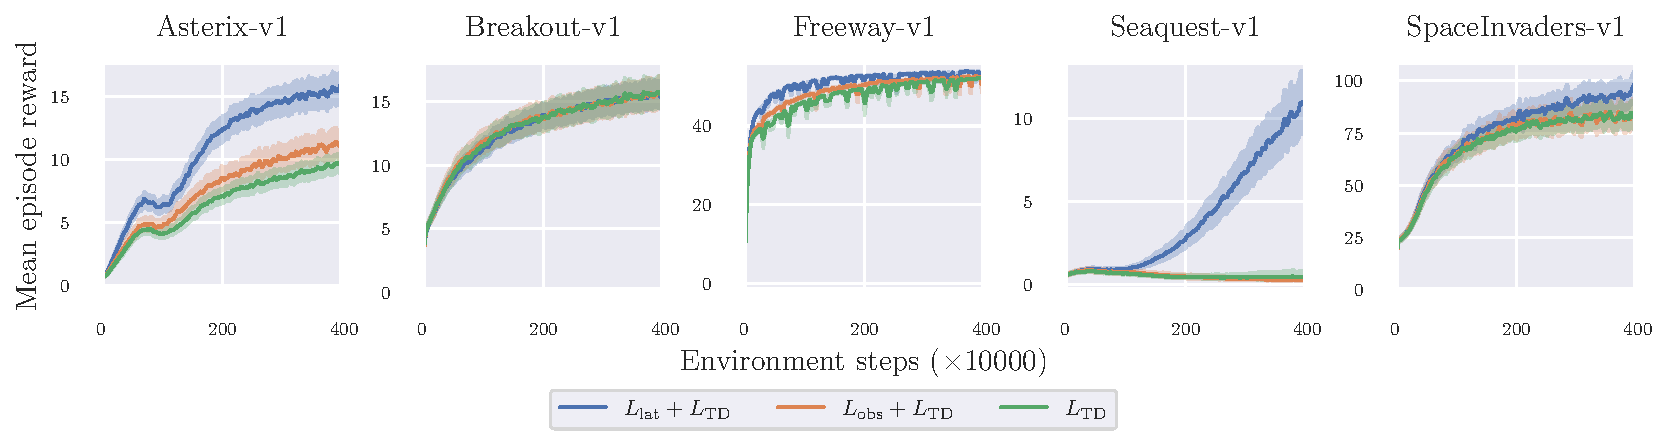
\includegraphics[width=\textwidth]{figures/understanding/rlc2024_minatar.pdf}
    \caption{Auxiliary task setup: Performance of all losses on the observation space as given without changes to the environment.}
    \label{fig:understanding:aux}
\end{figure}

\begin{figure}[t]
    \centering
    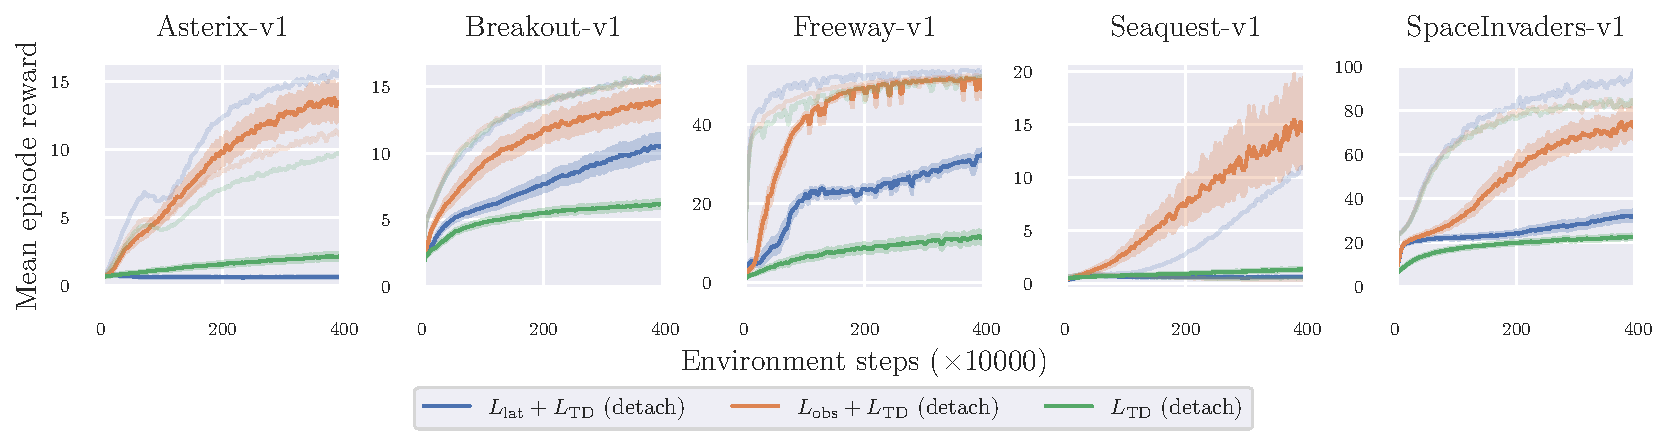
\includegraphics[width=\textwidth]{figures/understanding/rlc2024-detach_minatar.pdf}
    \caption{Stand-alone setup: Performance of all losses on the observation space as given without changes to the environment. The DQN baseline is using random features, which are not updated, to verify that learning features is indeed superior to a random feature baseline.}
    \label{fig:understanding:sta}
\end{figure}

\textbf{Auxiliary task learning vs general purpose feature learning (\autoref{fig:understanding:aux} and \autoref{fig:understanding:sta}):}
First, we compare both the auxiliary task and stand-alone feature learning scenarios.
As expected from prior work \parencite{jaderberg2016reinforcement,schwarzer2021dataefficient,farebrother2023protovalue}, in all cases using an auxiliary loss performs no worse (and often better) than vanilla DQN.
We find that as expected from \autoref{insight:understanding:3}, latent self-prediction is a stronger auxiliary loss function than observation reconstruction in three out of five environments.
However, when using the general-purposes losses alone, we clearly see observation reconstruction performing significantly better than latent self-prediction, which fails to learn any relevant features in several cases. This verifies \autoref{insight:understanding:1}.


Curiously, in the case of the Seaquest environment, we find that using observation prediction alone outperforms using it as an auxiliary task strongly, and performs on par with the auxiliary task variant of the latent self prediction loss.
Seaquest also has the sparsest reward structure in the test suite, which can make it a challenging environment for DQN. In this case, features based purely on the observed transition might allow for better policy learning.

This highlights that no algorithm is clearly superior in all settings and the reward and observation structure is very relevant for the performance of each loss.


\begin{figure}[t]
    \centering
    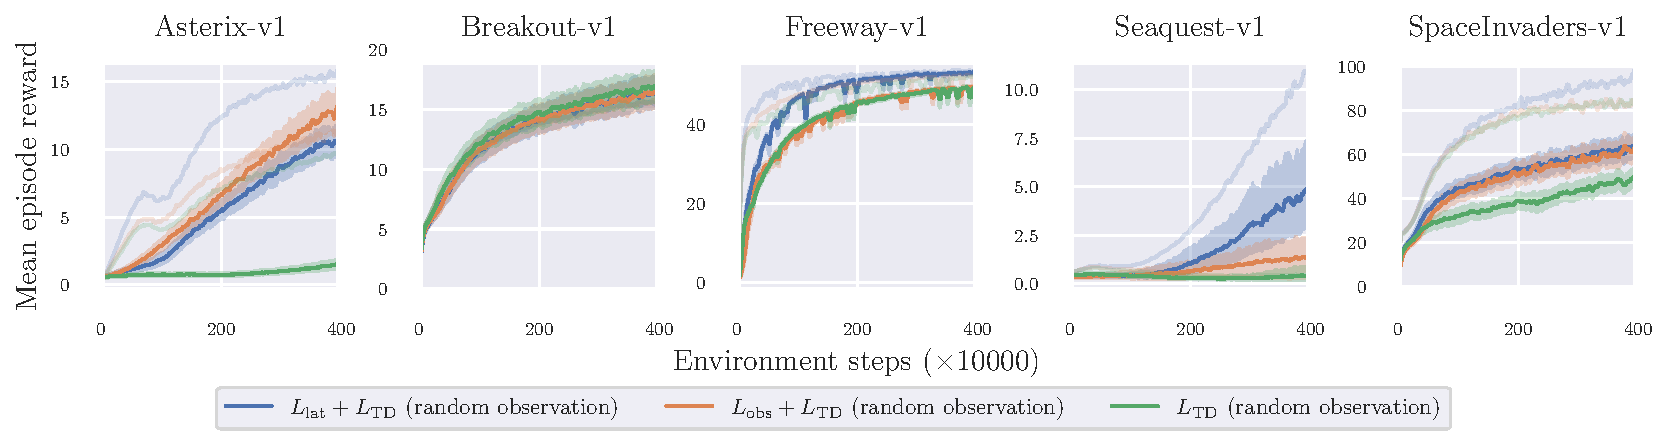
\includegraphics[width=\textwidth]{figures/understanding/rlc2024-distorted-fixed_minatar.pdf}
    \caption{Distorted observation function with a random transformation.}
    \label{fig:understanding:dist}
\end{figure}

\textbf{Observation space distortions (\autoref{fig:understanding:dist}):} To test the impact of changing the observation function, we sample a random binary matrix and multiply it to the flattened observation vector. We then reshape the observation to the original shape again.

All algorithms show themselves to be strongly impacted by this random observation distortions, which suggests that our claim of invariance of self-prediction relies too strongly on the linear gradient-flow limit.
This can in part be explained by the use of a convolutional layer in the standard baseline implementation of DQN which we adapted.
However, we still find that at least on two environments (Seaquest and Freeway), the latent self-prediction auxiliary task is able to recover more of the original performance than either observation prediction or DQN.
The DQN baseline seems to suffer the most from the introduction of the observation change, which suggests that correlations of the existing observation space play an important role in learning correct value function prediction.

Overall, we find that \autoref{insight:understanding:2} does not fully translate to the more complex test setting.
In part, this may be explained by the fact that the original observation spaces of the test environments already violate our assumptions for the one-hot encoding.
In addition, introducing linear correlation might not impact non-linear model learning in the same way it would impact linear models.
This highlights the need for more in-depth research on the interplay between given observation space and feature learning.

\begin{figure}[t]
    \centering
    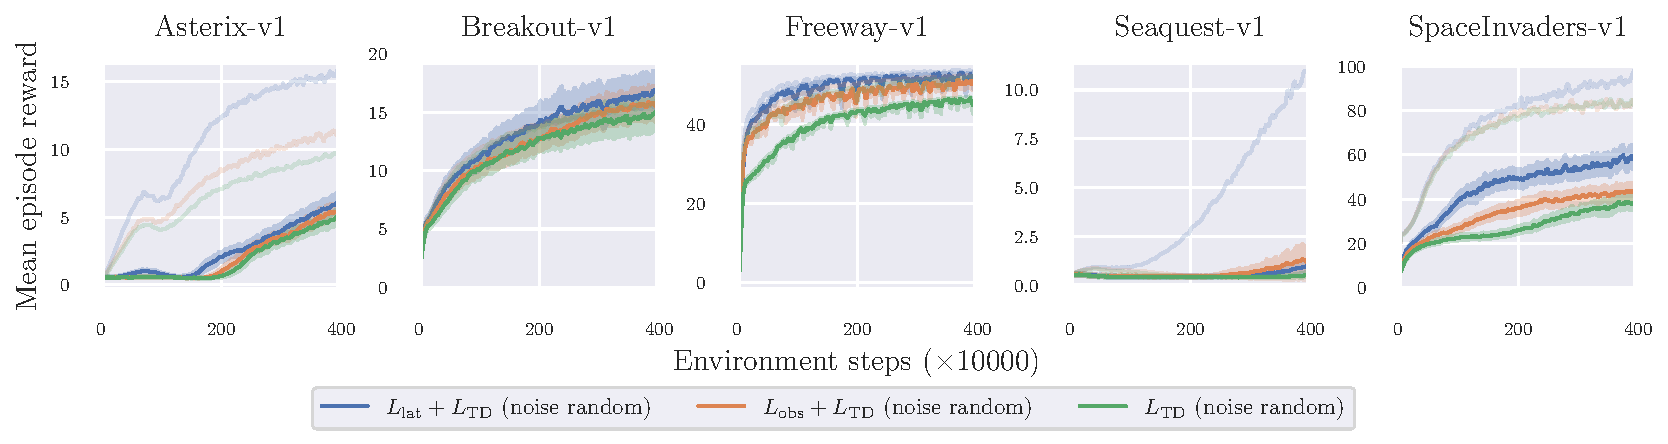
\includegraphics[width=\textwidth]{figures/understanding/rlc2024-noise-random_minatar.pdf}
    \caption{Appending random noise channels.}
    \label{fig:understanding:ran}
\end{figure}

\begin{figure}[t]
    \centering
    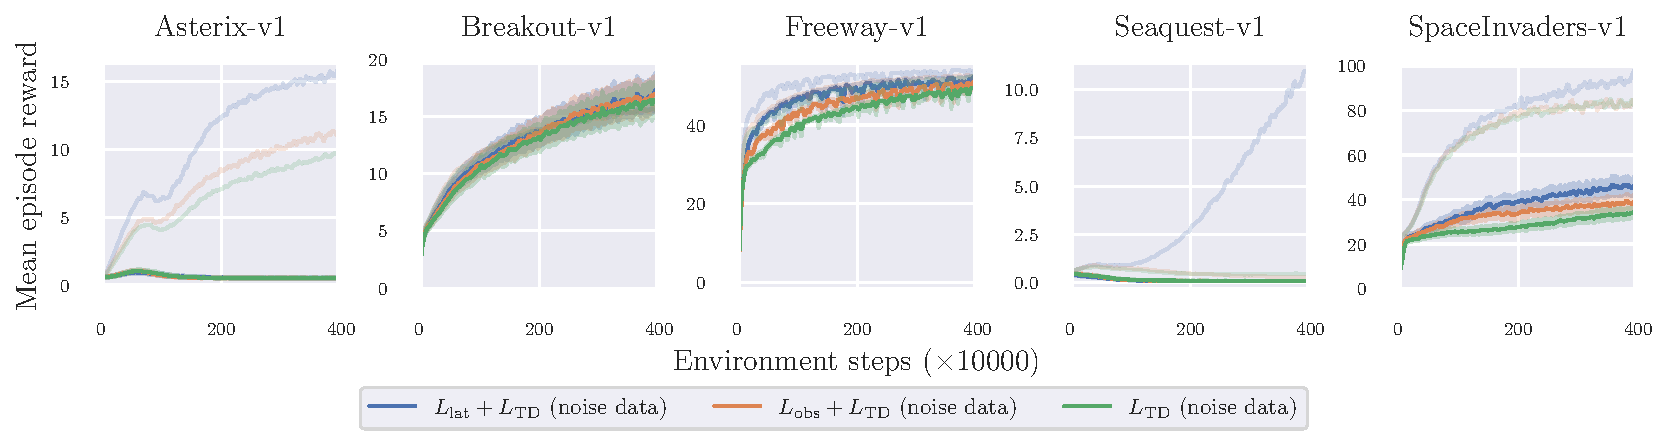
\includegraphics[width=\textwidth]{figures/understanding/rlc2024-noise-data_minatar.pdf}
    \caption{Appending structured noise channels using the Freeway environment.}
    \label{fig:understanding:dat}
\end{figure}

\textbf{Distractions (\autoref{fig:understanding:ran} and \autoref{fig:understanding:dat}):}
As our results are dependent on the spectral structure of the environment, different distraction models can be assumed to have differing impact on the efficacy of the tested losses.
This behavior is dependent on the structure of the noise.
If the distraction does not strongly change the top-$k$ singular or eigenspaces, it will be less problematic for the auxiliary tasks, especially for observation reconstruction.
Testing the impact of different distraction models on the top-$k$ spaces is out of scope for this work, but we conjecture that fully random noise has less structure than distractions following clear patterns.

Therefore, we consider two simple distraction models in our experiments. 
The distractions are concatenated to the original observations along the channel dimension.
First, we use random noise sampled independently for each state from a Bernoulli distribution.
As there is no predictable structure in this noise, we expect all algorithms to be able to deal with this distraction better.
Second, we choose one of the environments at random (Freeway-v1) and concatenate two copies to the observation space of each environment.
The dynamics are obtained by sampling a random action at each timestep independent from the policy and stepping the distraction environment with it.

We find a small advantage in some environments to using the latent self-prediction loss and using random noise, and no clear advantage from any algorithm in the structured noise case.
Structured noise poses a much larger challenge to most algorithms, completely preventing learning in several cases.
This partially validates that not only the presence or absence of noise matters, but also how it changes relevant quantities, e.g. the eigenvalues of the transition kernel.

In the continuous control experiments presented in \autoref{app:understanding:mujoco_results}, we find that the self-prediction loss performs generally better than in the MinAtar suite.
As the observation and reward structure differs between these two benchmark suite, this observation lends more credibility to our claims that the observation structure impacts the performance of algorithms.

\section{Conclusions}

When choosing an RL approach to use, practitioners are overwhelmed with a variety of loss function choices, without clear indication which one will be preferable in what scenario.
In our work, we introduce analytically tractable notions of distractions and observation functions.
With these we predict the performance of latent self-prediction and observation reconstruction as stand-along feature learning methods and auxiliary tasks, and study our theoretical insights empirically.
Our evaluation lends credibility to the use of simple surrogate models to obtain practically relevant insights into algorithmic performance.
However, in several cases we also find deviations between our predictions and more complex benchmarks.
Therefore, while we claim that our theoretical models have the ability to guide the choice of algorithms for applied settings, there is still a sizeable gap between theory and practice that remains to be bridged in future work.

We also note that our experiments showed substantial differences in behavior of auxiliary losses both within and across benchmarks and different noise distractions.
Previous work that studied the effect of distraction \parencite{nikishin2021control,voelcker2022value,ni2024bridging} did not discuss their distraction model in detail. 
In light of our results, we suggest that empirical research should be careful about the choice of benchmark and experimental setup and discuss the implications of the empirical setup explicitly.

On the empirical side the surprising effectiveness of the observation prediction loss on the Seaquest environment highlights the fact that even within benchmark suites, differences in the reward functions and observation models can lead to differing rankings between algorithms.
This further highlights the necessity of studying the structure of MDPs and to design algorithms that are robust to different structures, or adapt to them automatically.

Overall, we can conclude that model-based auxiliary tasks can be very helpful to structure latent representations in a way that complements the task of value function learning.
More importantly for the overall project of this thesis, we now have our first concrete example of an algorithm that leverages both a general-purpose method, predicting latent features, and a decision-aware method, in this case TD learning, and shows that there exists a synergy between these methods for stabilizing feature learning!

However, we have so far only used the model learning to stabilize the feature space.
Instead, we can also use the learned model itself to improve value function learning by generating additional data from the model in a Dyna style algorithm.
In the next chapter we will take a look at such model-based methods.
We will first investigate the idea of decision-aware learning in observation space models.
In the following chapter, we will show that combining latent self-prediction with decision-aware model learning greatly improves the stability of the IterVAML paradigm.